\documentclass[a4paper,twoside,10pt]{report}
% Richard Klein (2020,2021)

% Include Packages
%\usepackage[a4paper,inner=3.5cm,outer=2.5cm,top=2.5cm,bottom=2.5cm]{geometry}  % Set page margins
\usepackage{fullpage}
\usepackage{float}                  % Allows 'Here and Only Here' [H] for Floats
\usepackage{url}                    % \url{} command
\usepackage{charter}                  % Set font to Times
\usepackage{graphicx}               % \includegraphics
\usepackage{subfigure}              % Allow subfigures
\usepackage{amsmath}
\usepackage{amssymb}
\usepackage{amsthm}
\usepackage{booktabs}
\usepackage{parskip}
\usepackage[all]{nowidow}
\setnoclub[2]
\setnowidow[2]

% Referencing
% Provides \Vref and \vref to indicate where a reference is.
\usepackage{varioref} 
% Hyperlinks references
\usepackage[bookmarks=true,bookmarksopen=true]{hyperref} 
% Provides \Cref, \cref, \Vref, \vref to include the type of reference: fig/eqn/tbl
\usepackage{cleveref} 
% Setup Hyperref
\hypersetup{
  colorlinks   = true,              %Colours links instead of ugly boxes
  urlcolor     = blue,              %Colour for external hyperlinks
  linkcolor    = blue,              %Colour of internal links
  citecolor    = blue                %Colour of citations
}
% Names for Clever Ref
\crefname{table}{table}{tables}
\Crefname{table}{Table}{Tables}
\crefname{figure}{figure}{figures}
\Crefname{figure}{Figure}{Figures}
\crefname{equation}{equation}{equations}
\Crefname{equation}{Equation}{Equations}

% Wits Citation Style
\usepackage{natbib} % Force natbib.sty to put citation labels in the reference list
\makeatletter
\renewcommand\NAT@biblabel[1]{\def\citeauthoryear##1##2{##1 ##2}[#1]\hfill}
\renewcommand\NAT@bibsetup[1]{%
  \setlength{\itemsep}{\bibsep}\setlength{\parsep}{\z@}}
\def\@lbibitem[#1]#2{%
  \if\relax\@extra@b@citeb\relax\else
    \@ifundefined{br@#2\@extra@b@citeb}{}{%
     \@namedef{br@#2}{\@nameuse{br@#2\@extra@b@citeb}}}\fi
   \@ifundefined{b@#2\@extra@b@citeb}{\def\NAT@num{}}{\NAT@parse{#2}}%
   \item[\hfil\hyper@natanchorstart{#2\@extra@b@citeb}\@biblabel{#1}%
    \hyper@natanchorend]%
    \NAT@ifcmd#1(@)(@)\@nil{#2}}
\makeatother


\bibliographystyle{named-wits}
\bibpunct{[}{]}{;}{a}{}{}  % to get correct punctuation for bibliography
\setlength{\skip\footins}{1.5cm}
\newcommand{\citets}[1]{\citeauthor{#1}'s \citeyearpar{#1}}
\renewcommand\bibname{References}  

\pagestyle{headings}

\pagestyle{plain}
\pagenumbering{roman}

\renewenvironment{abstract}{\ \vfill\begin{center}\textbf{Aim}\end{center}\addcontentsline{toc}{section}{Abstract}}{\vfill\vfill\newpage}

\begin{document}
\onecolumn
\thispagestyle{empty}

\setcounter{page}{0}
\addcontentsline{toc}{chapter}{Preface}
\ 
\begin{center}
  \vfill
  {
  \huge \bf \textsc{Automatic License Plate Recognition}\\
  \large Digital Image Processing \\[20pt]
  \large School of Computer Science \& Applied Mathematics\\
  \large University of the Witwatersrand\\[20pt]
  \normalsize
  Molefe Molefe \\
  Tieho Ramphore \\
  1858893 \\[20pt]

  \today
  }

  \vfill
  \vfill
  
\includegraphics[width=1.5cm]{images/wits}
  \vspace{10pt}\\
  \small{Licene plate dketection and segmentation: Detect the license plate from an image of vehicle and perform segmentation}\\
\end{center}
\vfill
\newpage

\pagestyle{plain}
\setcounter{page}{1}

\phantomsection
\begin{abstract}
Design approaches that handle images taken in varying environments including but not limited to
\begin{itemize}
  \item Illumination Condition
  \item Non-Uniform Illumination
  \item Poor Illumination
  \item Different Weather Condition (Foggy, Rainy)
\end{itemize}
\end{abstract}



\phantomsection
\addcontentsline{toc}{section}{Table of Contents}
\tableofcontents
\newpage
\phantomsection
\newpage
\phantomsection
\newpage
\pagenumbering{arabic}

\chapter{Introduction}
Computer vision is a huge field in artificial intelligence responsible for teaching machines how to perceive and understand visual information.\
Our task is to use digital image processing techniques to detect vehicle license plates.\ 
These image processing techniques are comprised of sub-techniques that work cohesively to achieve the final result of a detected image.\ 
We present a novel method of capturing an image of a vehicle and returning the license plate ready for recognition.\ 
The subtask could be further reading the text presented from a localized license plate. \\ [4pt]

License plate detection can be used to track individuals that went above a certain speed;  allow or disallow access to restricted locations based on license plates.\ 
The applications of this technology are endless.

The difficulties of automatic license plate recognition(ALPR) we attempt to solve include but not limited to 
\begin{itemize}
  \item \textbf{Poor File Resolution}: Plate/Car is too far away
  \item \textbf{Poor Illumination}: The image is too dark or too bright 
  \item \textbf{Lack of Coordination}: The license plates are different for each country or state 
  \item \textbf{Environemnt}: The image contains foggy or rainy environments
\end{itemize}

\chapter{Related Work}
Papers from different countries face the problem of their algorithms being unable to detect foreign license plates.\ 
Some failures in recognition are due to different formats of the text written on the number plate or the plate having a different size.\ 
\citet*{redmon2016look} presented a method that captures the license plate of a vehicle. This paper placed cameras at suitable places and performed image processing techniques such as erosion,thinning and convolution to retrieve a license plate. \\ [4pt]

\citet*{RasheedAutomatedNP} proposed an ANPR method that recognizes Islamabad number plates by following two techniques: license plate locating using canny edge detection and hough transformation;  license number recognition using template matching.

\citet*{6510317} propsosed an algorithm that identifies a vehicle by its number plate considering skew detection.\
They perform number plate localization by combining methods such as thresholding and edge detection to perform prepare the image for hough rectangular transforms.\ 
We propose a method that uses contours to find the location of the license, instead they perform top-hat trasnformation and skew-detection to retrieve and fix the orientation of the license. 
The subtask of performing optimal character recognition(OCR) from a detected licesnse plate is performed by applying connected component analysis to segment the characters individually. Finally, they perform template matching for recognizing text using a statistical-based approach.
\chapter{Methodolgy}
We propose a novel method that will detect a number plate from an image.
License plates are relatively longer by width hence we approximated an aspect ratio between 4 and 6 to detect a rectangular object.

\begin{center}
  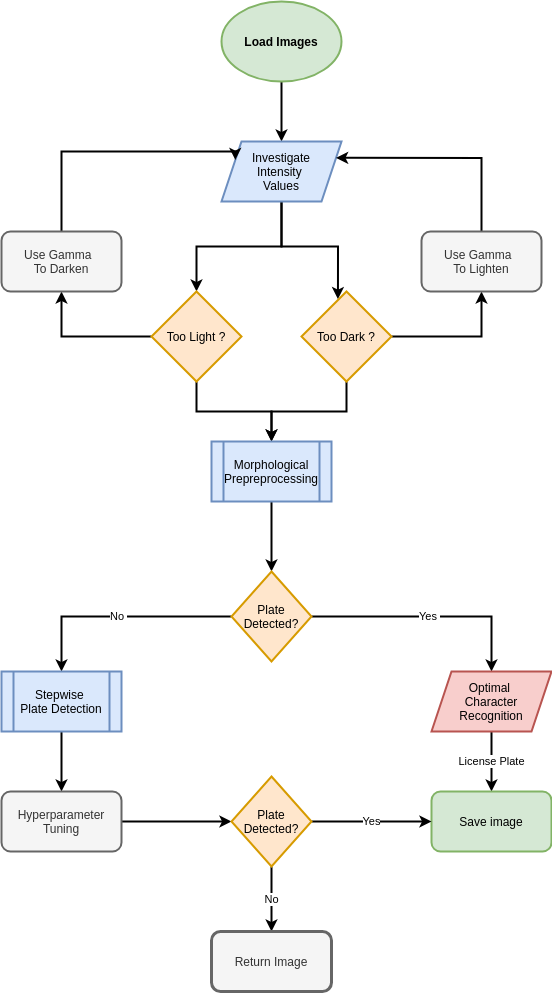
\includegraphics[width=11cm,height=15cm]{images/Methodology.png}
\end{center}

\section{Pre-Processing}
\subsection{Image Processing}
Image processing often requires converting the image into an 8-bit value representation.
We select one channel from a colored image by performing a grayscale operation.
It is necessary to assume that images are noisy and contain undesirable background information such as people, bicycles, etc.\
We blur the image using a gaussian blur to prepare it for edge detection.\ 
We would prefer that edge detection algorithm do not recognize insignificant image details.\

\subsection{Environemnt Handling}
// TODO

\subsection{Normalization}
// TODO 
\section{Number Plate Localization}

\subsection{Morphology}

We performed morphological operations that iteratively prepared the image for object segmentation.  \\[2pt]
\textbf{Black-Hat Morpohology}\\
We perform a black hat operation to reveal the dark regions on lighter backgrounds.\ 
This will highlight license plate numbers against the rest of the photo.\
 
\textbf{Closing}\\
We close the resulting operation to fill the small holes and identify larger structures in the image using a square kernel.\ 
We perform Otsu's threshold to reveal the light regions that may contain license plate characters.
\subsection{Edge Detection}
\textbf{Scharr Gradient}\\
We perform a Scharr gradient to detect edges in the image and highlight the boundaries surrounding a number plate. \\[3pt]
\textbf{Canny Edge Detection}\\
Preparing an image ready for optimal character recognition requires a clean license plate image.\
Canny edge detection computes the local gradient and edge direction at each point.\
The algorithm tracks along the top of the ridges created from finding the edge points.\
The ridge pixels are thresholded by a process called hysteresis thresholding and the algorithm performs edge linking by incorporating the weak pixels that are 8-connected to strong pixels.\
Non-maximum suppression is a technique that considers only the local maxima to be edges.\
Hysteresis thresholding forms longer edges by connecting weaker edge pixels to the strong edges.
Non-max suppresion filters objects of interest based on a thresholding criteria. [\href{https://towardsdatascience.com/non-maximum-suppression-nms-93ce178e177c}{TowardsDataScience}].
\begin{center}
  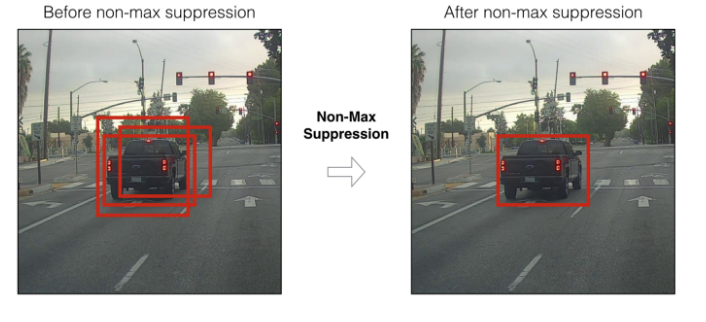
\includegraphics[width=10cm]{images/Non-maximum Suppression.png}
\end{center}
\subsection{Plate Orientation and Sizing}
// TODO 
\subsection{Contours}
Contours are curves joining continuous points that have the same color or intensity. It results in a closed figure that is bounded by the path of edges that have the same intensity.
Given the edge detected image, we have to find the contours that resemble a rectangular shape that has license plate characteristics.\ 
A ratio of 2:1 where the width is larger than the height closely approximates the dimensions of a license plate.\ 
We find the contours of the license plate candidates to retrieve the final license plate image.\ 
Contours generated by the OpenCV library randomly arrange their order.\ 
The contours that closely resemble the license plate are likely among the largest contours.\ 
Hence we sort the contours and find the contour with an aspect ratio resembling a rectangle.\ 
What remains is finding the location of the best contour and cropping the image at the relevant location. 
\begin{center}
  \begin{figure}[h!]
    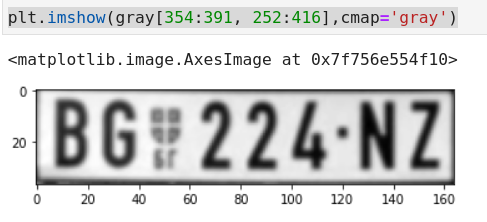
\includegraphics[width=10cm]{images/result.png}
    \caption{Taken from the notebook}
  \end{figure}
\end{center}
\subsection{Optimal Character Recognition}
 // TODO 

\chapter{Limitations}
\section{Automatic License Plate Recognition}
Automatic license plate recognition requires preliminary considerations as a prerequisite to detecting a number plate.\ 
The images need to be under controllable lighting conditions and contain recognizable license plates.\ 
Advanced ALPR methods utilize dedicated object detectors and state-of-the-art recurrent neural networks.\\ [4pt]

Another challenge is finding a dataset to train a custom ALPR algorithm. Government officials have security concerns regarding the deployment of unauthorized license plates for research purposes. Individuals prefer to keep their license plates hidden from public records. They are afraid that they would be susceptible to kidnapping and instances such as personal harm. 

ALPR datasets are difficult to curate because images need to be taken under consistent environments.
 
\chapter{Conclusion}
Computer vision is synonymous with surveillance, and as such computer vision algorithms solve security problems.\ 
Given that a person parks into a parking lot, we would be interested in discovering the time the individual arrived and the time they departed.\
Cameras are required to record video information that contains cars with license plates.\ 
We could place their detected license plates into a database and perform various searches for security reasons.\ 

A likely scenario is when a stolen vehicle is parked near cameras. And in this instance, automatic number plate recognition could quickly verify the location and time stamp of the vehicle.

\nocite{*}

\bibliography{references}\addcontentsline{toc}{chapter}{References}
\end{document}
